\documentclass[%
aps,
mph,%
amsmath,amssymb,
preprint,%
tightenlines,
%fleqn,
%notitlepage,
longbibliography,
superscriptaddress,
floatfix,
nofootinbib,
%author-year,%
%author-numerical,%
]{revtex4-2}

\linespread{1.2}

%\usepackage[draft]{graphicx} % Turns graphics off
\usepackage{nccmath}
\usepackage{setspace}
\usepackage{booktabs}
\usepackage{graphicx}
\usepackage[table,xcdraw,pdftex,dvipsnames]{xcolor}
\usepackage{dcolumn}% Align table columns on decimal point
\usepackage{bm}% bold math
\usepackage{siunitx}
%\usepackage[labelsep=colon]{caption}
\usepackage{subcaption}
\usepackage{amsmath}
\usepackage{amssymb}
\usepackage{amsthm}
\usepackage{booktabs}
\usepackage{array}
\usepackage{multirow} 
\usepackage{nicematrix} %alternative to multirow...?
\usepackage{ragged2e}
\usepackage{textcomp}
\usepackage{enumitem}
\usepackage{mathtools}
\usepackage{hyperref}
\usepackage[toc,page]{appendix}
\usepackage{lipsum}
\usepackage{cleveref} % for references like \cref{X,Y,Z}
\usepackage[T1]{fontenc} %accents and other stuff for letters
\usepackage{comment}

% stuff for boxing in tables
\usepackage{tikz}
\usetikzlibrary{fit,shapes.misc}

\renewcommand\qedsymbol{$\blacksquare$}

\DeclareCaptionStyle{mystyle}
  {format=plain,%
  %textformat=period,
    justification=raggedright,
    singlelinecheck=false, % when true, captions are centered
  }% all captions are left aligned
\captionsetup{justification=raggedright,singlelinecheck=false} % need this too for some reason even though the above says the same thing? I'll fix this later -12/1/2023

\newcommand\marktopleft[1]{%
    \tikz[overlay,remember picture] 
        \node (marker-#1-a) at (0.4,1.65ex) {};%
}
\newcommand\markbottomright[1]{%
    \tikz[overlay,remember picture] 
        \node (marker-#1-b) at (0,0) {};%
    \tikz[overlay,remember picture,thick,dashed,inner sep=3pt]
        \node[draw,rounded rectangle,fit=(marker-#1-a.center) (marker-#1-b.center)] {};%
}

\newcommand{\mysize}{0.6} %for changing figure sizes
\newcommand{\myrowsep}{1.25} %for changing row separations in tables
\newcommand{\mytablefontsize}{\footnotesize} 
% https://tex.stackexchange.com/questions/56008/different-sizes-of-font-available-in-table

\newcolumntype{L}{>{$}l<{$}}
\newcolumntype{C}{>{$}c<{$}}
\newcolumntype{R}{>{$}r<{$}}
\newcommand{\nm}[1]{\textnormal{#1}}
  

%\bibliographystyle{apsrev4-2}% cannot be on and with longbibliography at the same time :/

\usepackage{etoolbox}
\patchcmd{\section}
  {\centering}
  {\raggedright}
  {}
  {}
\patchcmd{\subsection}
  {\centering}
  {\raggedright}
  {}
  {}

\renewcommand{\andname}{\ignorespaces}

\begin{document}

\title{Shielding Project Report - MPHY 397}


\author{Raj Tummala}
\affiliation{The University of Chicago, Chicago, IL, USA}

\author{Rob Tomek}
\affiliation{The University of Chicago, Chicago, IL, USA}

\author{Amy Renn\'{e}}
\affiliation{The University of Chicago, Chicago, IL, USA}
\affiliation{Argonne National Laboratory, Lemont, IL, USA}

\author{JP Phillips}
\affiliation{The University of Chicago, Chicago, IL, USA}

\author{Lucas Berens}
\affiliation{The University of Chicago, Chicago, IL, USA}

\maketitle

%\date{\today}% It is always \today, today,
             %  but any date may be explicitly specified

\section{Introduction}
\section{LINAC Primary and Secondary Barriers}
\section{LINAC Maze and CT Simulation}
    \subsection{Problem Description and Assumptions}
        A $\SI{350}{mm} \times \SI{350}{mm}$ CT sim control room is adjacent to a $\SI{700}{mm} \times \SI{550}{mm}$ CT sim vault. Workload and CT specifications are depicted in Table \ref{CT_spec}. Considering the facility is on a single level, floor and ceiling shielding is not required. Additionally, we assume the facility is not in proximity to any sidewalks with pedestrian traffic, negating the need for external wall shielding. The only remaining walls to consider is that adjacent to the LINAC room and the sim vault.
        
        Because the LINAC room already has shielding in place capable of protecting against therapeutic-level scattered radiation, these measures will far surpass any dose from the CT which primarily outputs only scattered and leakage (secondary) radiation from gamma beams of \SI{80}{keV} or \SI{140}{keV}. Therefore, the only wall requiring shielding is the wall adjacent to the CT sim room. It is worth mentioning that there is a storage room on the same wall as the sim room, but given that this room is rarely occupied and only for very short periods at a time, shielding is not required here. The following calculations estimate the required shielding thickness for the CT sim room following the CTDI method described in the NCRA Report 147 \cite{national2004ncrp}. 

        \bgroup
        \def\arraystretch{\myrowsep}
        \setlength{\tabcolsep}{20pt}
        \begin{table*}[h!] % table for one column, table* for 2 columns 
        \mytablefontsize
        \captionsetup{style=mystyle}
        \captionof{table}{CT facility workload and specifications.}
        \centering
        %\resizebox{0.7\textwidth}{!}{%
        %\begin{tabular}{p{1.3cm} llccrl
        \begin{tabular}{lcc
        >{\columncolor[HTML]{FFF}}c }
        \hline
        \multicolumn{1}{c}{Parameter} & \multicolumn{1}{c}{Body} & \multicolumn{1}{c}{Head} 
        \\
        \hline\hline
        Patients/Week & 50 & 10 \\ 
        \% Requiring CT & 50 & n/a \\ 
        X-Ray Energy (keV) & 140 & 80 \\ 
        Imaging Length (cm) & 50 & 20 \\
        mAs & 350 & 200 \\ 
        Pitch & 1.3 & 1.0 \\ 
        $_nCTDI_{100}$ & 0.14 & n/a \\
        \hline\hline
        \end{tabular}%
        \label{CT_spec}
        \end{table*}
        \egroup 
    
    \subsection{Secondary Air-Kerma Values per Patient at 1\hspace{0.85pt}m}
        NCRP defines the secondary air-kerma value per patient at \SI{1}{m} ($K^1\mathrm{_{sec}}$) by
        \begin{align} \label{k_patient}
                K^1\mathrm{_{sec}} = \left(\kappa\right) \left( \frac{L}{P}\right) \left(\mathrm{mAs}\right) \left(_n\mathrm{CTDI}_{100}\right)
        \end{align}
        where $\kappa$ is the scatter fraction per centimeter, $L$ is the imaging length, and $P$ is pitch. $\kappa$ values for body and head CTs provided by the NCRP are $\kappa\mathrm{_{body}} = \SI{3e-4}{\per \cm}$ and $\kappa\mathrm{_{head}} = \SI{9e-5}{\per \cm}$, respectively.  

        In the case of the missing $_n\mathrm{CTDI}_{100}$ value for head scans (see Table \ref{CT_spec}), we take the reference value provided in the NCRP report and assume $_n\mathrm{CTDI}_{100}\text{(Head)} = \qty[mode = text]{0.223}{mGy.mAs^{-1}}$. Because the calculation is more heavily dependent on the $\kappa\mathrm{_{body}}$ value which is larger than $\kappa\mathrm{_{head}}$ by an order of magnitude, this assumption is justified. Substituting values for body or head CTs from Table \ref{CT_spec}, the following $ K^1\mathrm{_{sec}}$ values are obtained:
        \begin{align*}
            K^1\mathrm{_{sec}(Body)} &= \left(\SI{3e-4}{\per \cm}\right)\left(\frac{\SI{50}{cm}}{1.3}\right)(\SI{350}{mAs})\left(\qty[mode = text]{0.14}{mGy.mAs^{-1}.patient^{-1}}\right) \\
            &= \SI{0.5654}{mGy/patient}\\
            K^1\mathrm{_{sec}(Head)} &= \left(\SI{9e-5}{\per \cm}\right)\left(\frac{\SI{20}{cm}}{1}\right)(\SI{200}{mAs})\left(\qty[mode = text]{0.223}{mGy.mAs^{-1}.patient^{-1}}\right) \\
            &= \SI{0.0803}{mGy/patient}
        \end{align*}

    \subsection{Total Secondary Air-Kerma Value at 3\hspace{0.85pt}m}
        Given 50\% of body CT patients required a CT scan, the total number of body CT patients is $n\mathrm{_{body}} = 50\cdot0.5 = 25$. Because a percent requiring scan value is not given for head patients, we consider the maximum possible dose case according to ALARA principles and assume 100\% of head CT patients require a scan ($n\mathrm{_{head}} = 10$). Therefore, the total secondary air-kerma value at a distance $d$ away from the shielding wall, accounting for the upper limit workload from both body and head scans and the inverse square law, is shown in Equation (\ref{k_total}). 

        \begin{equation}\label{k_total}
            K\mathrm{_{sec}} = \left(\frac{\qty{1}{m}}{d}\right)^2 [n\mathrm{_{body}}\cdot K^1\mathrm{_{sec}(Body)}) + n\mathrm{_{head}}\cdot K^1\mathrm{_{sec}(Head)}]
        \end{equation}
        
        From the floor plan, it can be seen that the isocenter of the CT is roughly 3 m from the surface of the sim wall. Substituting values and solving: 
        \begin{align*}
            K\mathrm{_{sec}} &= \left(\frac{\qty{1}{m}}{\qty{3}{m}}\right)^2\left[\left(\qty{25}{\frac{patients}{week}}\right)\left(\SI{0.05654}{\frac{mGy}{patient}}\right)+ \left(\qty{10}{\frac{patients}{week}}\right)\left(\SI{0.0803}{\frac{mGy}{patient}}\right)\right]\\
            &= \SI{1.66}{mGy/week}
        \end{align*}
        
    \subsection{Required Shielding Thickness}
            According to ICRP guidance, the annual occupational dose limit is \qty{50}{mGy/year}. Assuming a 40 week work year, the weekly dose limit for workers in the CT sim control room $\frac{\qty{50}{mGy/year}}{\qty{40}{week/year}}$ = \qty{1.25}{mGy/week}. We assume the sim room is a controlled area (no public access), and restricted to radiation workers only. Therefore, the required barrier transmission is calculated as:
        \begin{equation*}
            B = \frac{\qty{1.25}{mGy/week}}{\qty{1.66}{mGy/week}} = 0.7531
        \end{equation*}
        
        Substituting $B$ into Equation A.3 in Appendix 2 of NCRP 147 using the fit parameters $\alpha, \beta, \gamma$ provided for lead shielding of \qty{140}{kVp} CT scanners, the required barrier lead thickness $x\mathrm{_{lead}}$ is calculated as:
        
        \begin{align*}
            x\mathrm{_{lead}} &= \frac{1}{\alpha\gamma}\ln\left(\frac{B^{-\gamma}+\frac{\beta}{\alpha}}{1+ \frac{\beta}{\alpha}} \right)\\
            x\mathrm{_{lead}} &= \frac{1}{\qty{2.009}{mm^{-1}}\cdot0.342}\ln\left(\frac{( 0.7531)^{-0.342}+\frac{\qty{3.99}{mm^{-1}}}{\qty{2.009}{mm^{-1}}}}{1+ \frac{\qty{3.99}{mm^{-1}}}{\qty{2.009}{mm^{-1}}}} \right)\\
            &= \qty{0.05}{mm}
        \end{align*}
        
        Similarly, by substituting fit parameters for concrete shielding of 140 kVp CT scanners, the required barrier lead thickness $x\mathrm{_{concrete}}$ is calculated as:
        \begin{align*}
            x\mathrm{_{concrete}} &= \frac{1}{\qty{0.0336}{mm^{-1}}\cdot0.519}\ln\left(\frac{( 0.7531)^{-0.519}+\frac{\qty{0.0122}{mm^{-1}}}{\qty{0.0336}{mm^{-1}}}}{1+ \frac{\qty{0.0122}{mm^{-1}}}{\qty{0.0336}{mm^{-1}}}} \right)\\
            &= \qty{6.31}{mm}
        \end{align*}
        
        Therefore, according to the CTDI method, the required shielding for the CT sim room is \SI{0.05}{mm} lead, or equivalently, \SI{6.31}{mm} concrete. Since \SI{0.05}{mm} lead is much less than the 1.59 mm lead thickness standard, \SI{1.59}{mm} shielding is confirmed to be a safe and appropriate barrier for the CT sim room barrier.
        
    \subsection{DLP Calculation Check} 
        NCRP 147 also provides a secondary CT shielding calculation based on dose length product (DLP) values. The method is similar to CTDI in all but the $K^1\mathrm{_{sec}}$ calculation which is defined according to Equation (\ref{DLP}) where the DLP values are \SI{550}{mGy.cm} and \SI{1200}{mGy.cm}, for body and head CT scans, respectively (NCRP 147, Table 5.2 \cite{national2004ncrp}).
        \begin{align}\label{DLP}
            K^1\mathrm{_{sec}({Body})} &= 1.2 \cdot \kappa\mathrm{_{body}} \cdot \mathrm{DLP}\\
            K^1\mathrm{_{sec}(Head)} &= \kappa\mathrm{_{body}}\cdot \mathrm{DLP}
        \end{align}
        
        Following the methodology outlined in earlier sections and substituting in known values, the required barrier thicknesses via DLP is calculated as follows. 
        \begin{equation}
        \begin{aligned} \nonumber
            K^1\mathrm{_{sec}({Body})} &= 1.2 \left(3 \times 10^{-4}\right) (550) \\
            &= \qty{0.1980}{mGy/patient}\\ \\
            K^1\mathrm{_{sec}({Head})} &= \left(9 \times 10^{-5} \right) (1200) \\
            &= \qty{0.1080}{mGy/patient}\\ \\
            \implies K\mathrm{_{sec}} &= \left(\frac{\qty{1}{m}}{\qty{3}{m}}\right)^2  \left[ \left( \qty{25}{\frac{patients}{week}}\right)\left(\SI{0.1980}{\frac{mGy}{patient}}\right)+ \right.\\
            & \hspace{63.25pt} \left.\left(  \qty{10}{\frac{patients}{week}}\right)\left(\SI{0.1080}{\frac{mGy}{patient}}\right) \right]\\
            &= \qty{6.14}{mGy/week}\\ \\
            \implies B &= \frac{\qty{1.25}{mGy/week}}{\qty{6.14}{mGy/week}} \\
            &= 0.2035
        \end{aligned}
        \end{equation}
        
        
        \begin{align*}
            x\mathrm{_{lead}} &= \frac{1}{\qty{2.009}{mm^{-1}}\cdot0.342}\ln\left(\frac{( 0.2035)^{-0.342}+\frac{\qty{3.99}{mm^{-1}}}{\qty{2.009}{mm^{-1}}}}{1+ \frac{\qty{3.99}{mm^{-1}}}{\qty{2.009}{mm^{-1}}}} \right) = \qty{0.32}{mm}\\
            x\mathrm{_{concrete}} &= \frac{1}{\qty{0.0336}{mm^{-1}}\cdot0.519}\ln\left(\frac{( 0.2035)^{-0.519}+\frac{\qty{0.0122}{mm^{-1}}}{\qty{0.0336}{mm^{-1}}}}{1+ \frac{\qty{0.0122}{mm^{-1}}}{\qty{0.0336}{mm^{-1}}}} \right) = \qty{38.07}{mm}
        \end{align*}
        
        It can be seen that the DLP method results in a higher total secondary air-kerma estimate of 6.14 mGy/week compared to the $_n\mathrm{CTDI}_{100}$ method estimation of \qty{1.66}{mGy/week}. Even with this factor of $\sim$4 difference, the conservative DLP method still results in a lead thickness of only \qty{0.32}{mm} (or \qty{38.07}{mm} concrete thickness) which is smaller than the shielding standard of \qty{0.59}{mm}. This calculation confirms the CTDI result that standard shielding practices utilizing a \qty{0.59}{mm} lead barrier are appropriate for the CT sim room investigated. 

\section{Brachytherapy Room and Maze}
    \subsection{Does the decrease in activity from \SI{10}{Ci} to \SI{5}{Ci} impact the workload of treating 20 patients per week, with an average treatment time of 5 minutes per patient, using the new source?}
    We calculate the workload using
    \begin{align}
        W &= f A \Gamma_x t_w,
    \end{align}
    where $W$ is the workload, $f = \qty{1}{cGy/R.m^2}$ and relates R to cGy, $A$ is the source strength/activity, $\Gamma_x = \SI{0.48}{R.m^2/Ci.hr}$ is the exposure rate constant for $^{192}\mathrm{Ir}$, and $t_w = \left( \qty{20}{patients/week} \right)\left(\qty{5}{min}\right) = \qty{1.67}{hr}$ is the integrated treatment time per week for all patients. For a source strength of \SI{10}{Ci}, we have,
    \begin{align*}
        W &= \left(\qty{1}{cGy/R.m^2}\right)(\left( \SI{10}{Ci} \right) \left( \SI{0.48}{R.m^2/Ci.hr} \right) \left( \qty{1.67}{hr/week} \right) \\
        &= \qty{8.00}{cGy/week}.
    \end{align*}
    Now, we assume that the transmission through the patient is 20\%, giving a total workload of \qty{1.60}{cGy/week}. With $A = \SI{5}{Ci}$, this is halved to be $W = \qty{0.80}{cGy/week}$, however a lower source activity also means that treatment times are longer to deliver the same patient dose, so the workload would not actually change.

    \subsection{Determine the necessary lead shielding for all barriers.}
    Here we use the barrier transmission factor $B$,
    \begin{align}
        B = \frac{Pd^2}{WTU},
    \end{align}
    where $P = \qty{0.02}{mSv/week}$ is the dose allowed in the room for an uncontrolled area, or $P = \qty{0.1}{mSv/week}$ $d$ is the distance from the source to the wall, $W$ is the workload calculated earlier, $T$ is the occupancy factor, and $U$ is the use factor. We consider here the north (N), east (E), south (S), and western (W) walls with distances from the source of $d_\mathrm{N} = \qty{1.5}{m}$, $d_\mathrm{E} = \qty{1.0}{m}$, $d_\mathrm{S} = \qty{4.5}{m}$, $d_\mathrm{W} = \qty{3.75}{m}$. $B_i$ is then:
    \begin{align*}
        B_{\mathrm{N}} &= \frac{\left(\qty{0.01}{cGy/week}\right)\left(\qty{1.5}{m}\right)^2}{\left(\qty{1.60}{cGy/week}\right)\left(1.0\right)\left( 1 \right)}\\
        &= \qty{0.141}{m^2} \\ \\
        B_{\mathrm{E}} &= \frac{\left(\qty{0.002}{cGy/week}\right)\left(\qty{1.0}{m}\right)^2}{\left(\qty{1.60}{cGy/week}\right)\left(0.25\right)\left( 1 \right)}\\
        &= \qty{0.005}{m^2} \\ \\ 
        B_{\mathrm{S}} &= \frac{\left(\qty{0.002}{cGy/week}\right)\left(\qty{4.5}{m}\right)^2}{\left(\qty{1.60}{cGy/week}\right)\left(0.50\right)\left( 1 \right)}\\
        &= \qty{0.506}{m^2} \\ \\ 
        B_{\mathrm{W}} &= \frac{\left(\qty{0.01}{cGy/week}\right)\left(\qty{3.75}{m}\right)^2}{\left(\qty{1.60}{cGy/week}\right)\left(0.50\right)\left( 1 \right)}\\
        &= \qty{0.176}{m^2} \\ \\ 
    \end{align*}
    Now we simply find the thickness of the required lead via Figure \ref{lead_thicc}, taken from the NCRP 49 report \cite{simmons1978structural}. We find that the thicknesses of lead, $T_{i}$, for each wall are $T_\mathrm{N} = \qty{3.6}{cm}$, $T_\mathrm{E} = \qty{2.4}{cm}$, $T_\mathrm{S} = \qty{1.4}{cm}$, $T_\mathrm{W} = \qty{1.8}{cm}$. The western wall, however, will have shielding for the LINAC, which is thicker than the required amount for brachytherapy. 
    \begin{figure}[h!]
        \centering
        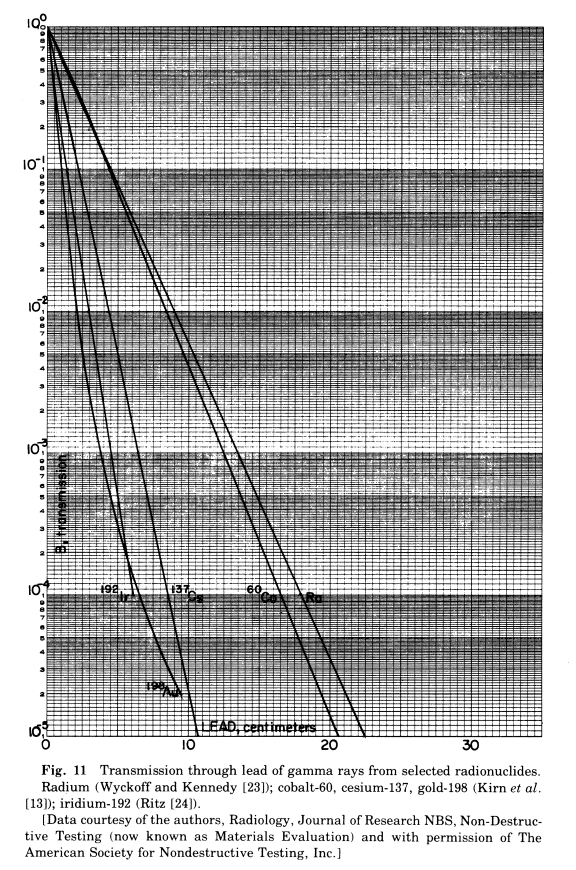
\includegraphics[width=0.75\linewidth]{figures/image.png}
        \label{lead_thicc}
    \end{figure}

    
\section{Conclusion}

\bibliography{bib}
\end{document}
